% ============================================================================
%  CAMBIOS PARA LA TESIS  (MIA-thesis-11.tex)
%  Todo en UTF-8 limpio. Cada bloque indica DÓNDE va en tu documento.
%  No reescribo tu prosa: solo reemplazo/inserto lo que pediste.
%
%  Requisitos de preámbulo (YA los tienes todos): tikz, xcolor, graphicx,
%  subcaption, listings, booktabs, float. No hace falta añadir paquetes.
% ============================================================================


% ============================================================================
%  BLOQUE 1 — ITERACIÓN 5 (CORRECCIÓN)
%  REEMPLAZA el párrafo que empieza por "El usuario interactúa enviando su
%  prompt o archivo de texto al \texttt{LLMBuilder}." JUNTO CON la figura
%  iteration5.png (fig:seq_iter5) por TODO lo siguiente:
% ============================================================================

El usuario interactúa enviando su descripción en lenguaje natural al
\texttt{LLMBuilder}. El servicio que ofrece este módulo es la ``producción''
material de los artefactos de entrada requeridos por la Iteración~3: un archivo
de configuración declarativo (\texttt{config.toml}), que delimita el espacio y
los estados, y, cuando la simulación lo requiere, un archivo de lógica
imperativa (\texttt{rules.jl}) con las matemáticas del modelo. A diferencia de
una única consulta al modelo, el \texttt{LLMBuilder} encadena varias llamadas
—clasificación, generación y reparación— y, una vez obtenidos y validados los
artefactos de forma transparente, los entrega al módulo \texttt{Initialization}
y lanza la simulación, sin que el usuario haya escrito una sola línea de lógica
algorítmica. La Figura~\ref{fig:seq_iter5} detalla esta orquestación.

\begin{figure}[H]
\centering
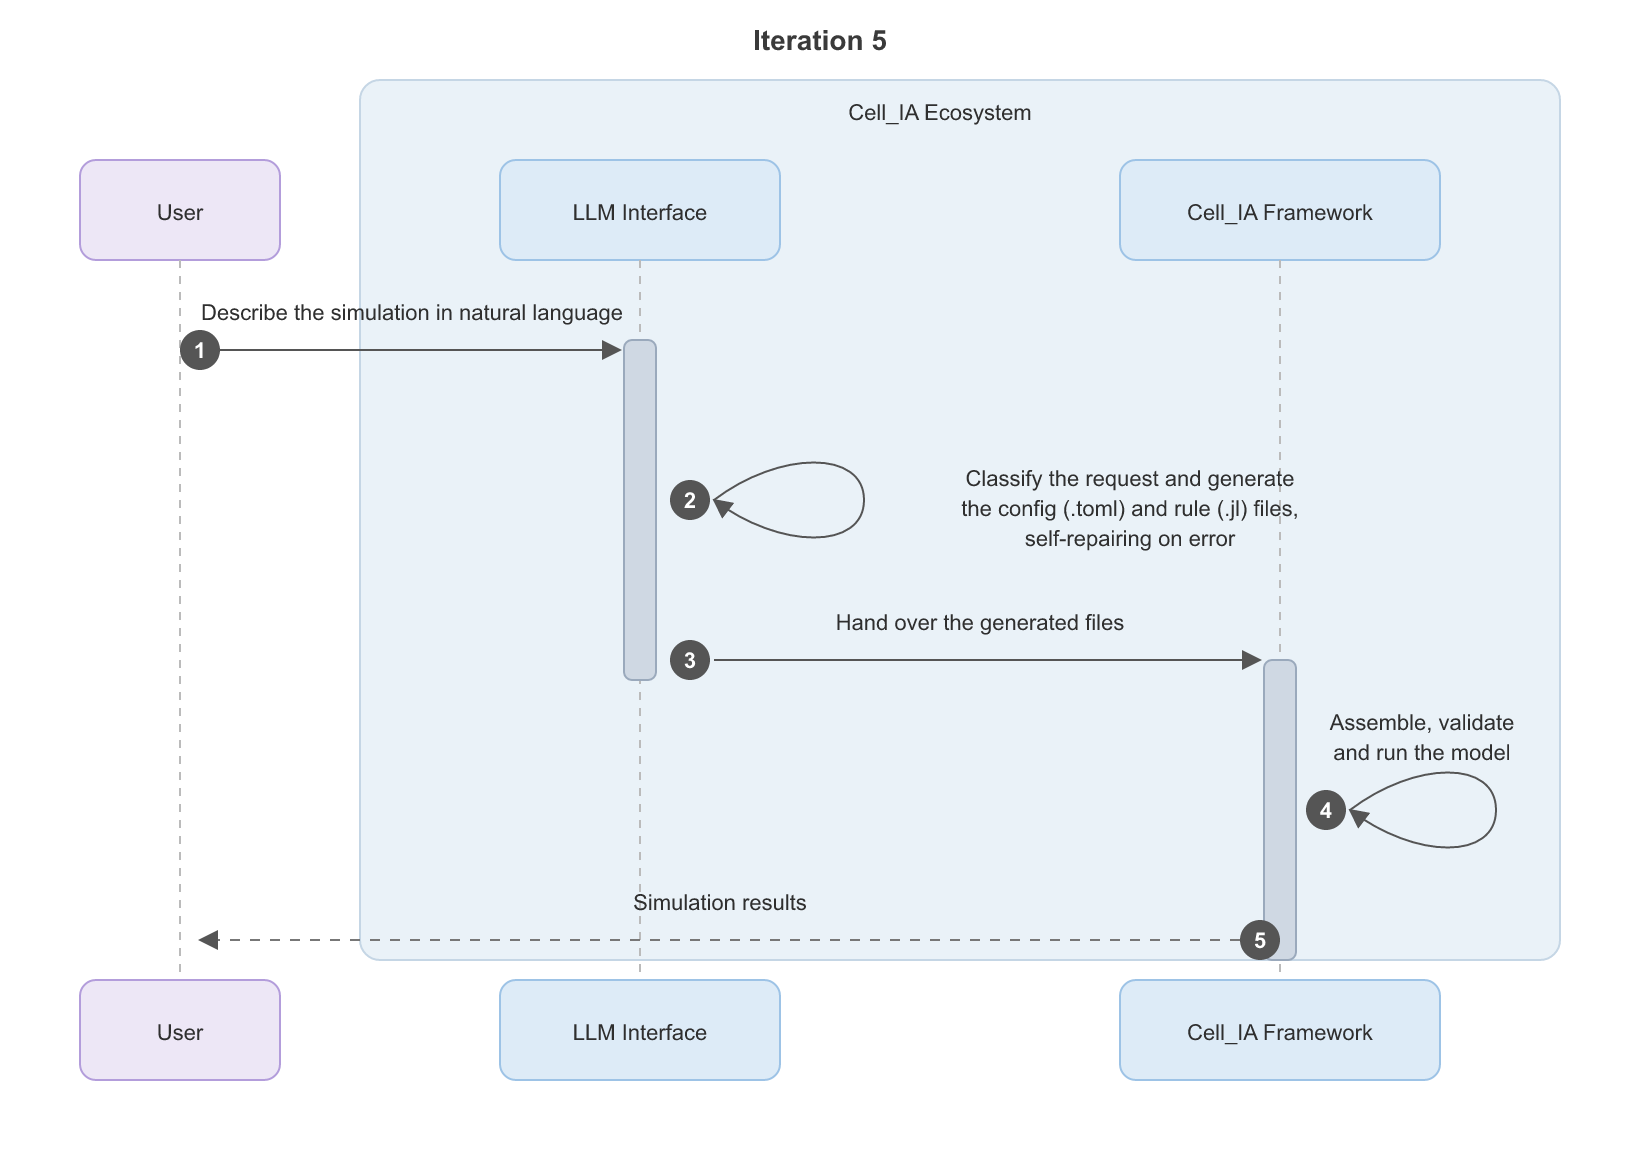
\includegraphics[width=1\textwidth]{iteration5.png}
\caption{Diagrama de secuencia, simplificado, de la generación de simulaciones mediante el LLM. El usuario describe la simulación en lenguaje natural; la interfaz con el modelo de lenguaje clasifica la petición (\emph{router}) y genera los archivos de configuración (\texttt{.toml}) y de reglas (\texttt{.jl}), reparándolos automáticamente ante errores de validación o de ejecución; por último, el framework Cell\_IA ensambla, valida y ejecuta el modelo y devuelve los resultados al usuario.}
\label{fig:seq_iter5}
\end{figure}


% ============================================================================
%  BLOQUE 2 — ITERACIÓN 5 (CORRECCIÓN)
%  REEMPLAZA por completo el \subsubsection "Estrategia de prompt engineering..."
%  DESDE su \subsubsection HASTA justo ANTES del párrafo que empieza por
%  "No obstante, dado que el modelo de lenguaje opera estrictamente como una
%  función de texto a texto..." (ese párrafo del harness se CONSERVA tal cual).
% ============================================================================

\subsubsection{Estrategia de \textit{prompt engineering} y orquestación de software (\textit{harness engineering})}
\label{sec:prompt_eng}
La interacción con el LLM no se apoya en un único prompt monolítico ni en
\textit{fine-tuning} del modelo, sino en una arquitectura de \textbf{varios
prompts especializados} coordinados por una capa de orquestación
(\textit{harness}) que encadena clasificación, generación y reparación
automática. Este diseño reutiliza el mismo modelo base para cualquier simulación
sin modificar sus pesos y se estructura en los siguientes niveles:

\begin{enumerate}
    \item \textbf{Prompt de enrutado (\textit{router}):} La primera llamada al
    modelo no genera código, sino que \textit{clasifica} la petición del usuario
    en una de cuatro categorías de simulación: rejilla discreta
    (\texttt{grid\_discrete}), campo continuo tipo Lenia
    (\texttt{continuous\_field}), espacio continuo de agentes móviles
    (\texttt{continuous\_space}) y rejilla hexagonal (\texttt{hexagonal}). Para
    garantizar que la respuesta sea siempre interpretable por el sistema, esta
    llamada se restringe mediante una \textbf{gramática formal} (en notación
    GBNF) que obliga al modelo a emitir exclusivamente un objeto JSON con la
    categoría elegida. La separación es deliberada: un modelo pequeño
    (1.5\,B de parámetros) acierta mucho más resolviendo primero ``qué tipo de
    problema es'' que afrontando a la vez la clasificación y la generación.
    \item \textbf{Megaprompt específico de categoría:} Una vez fijada la
    categoría, la generación se realiza con un \textit{prompt} de sistema
    compuesto por dos piezas: un \textbf{núcleo común} (\texttt{common\_core}),
    que fija el formato de salida, las secciones obligatorias del
    \texttt{config.toml} y las reglas universales de la API de Agents.jl; y un
    \textbf{bloque específico} de la categoría, que detalla el tipo de espacio,
    el tipo de estado, las reglas \textit{built-in} ya disponibles, los
    identificadores que deben copiarse de forma literal y ejemplos completos.
    Existe, por tanto, un megaprompt distinto por cada categoría, especializado
    en sus restricciones, en lugar de un único prompt genérico que debía cubrir
    todos los casos simultáneamente.
    \item \textbf{Confirmación interactiva:} Antes de generar, el sistema muestra
    al usuario una descripción depurada de la categoría seleccionada y le permite
    aceptarla, rechazarla —lo que descarta esa categoría y vuelve a enrutar— o
    matizarla con una aclaración —que se reincorpora a la petición y re-enruta
    sin descartar la categoría—. Así, las correcciones sucesivas del usuario
    refinan el enrutado sin contradecirse.
    \item \textbf{Bucle de reparación por validación:} Los archivos generados se
    someten a una \textbf{validación estática} (sin ejecutar Julia) que comprueba
    que el \texttt{config.toml} es sintácticamente válido, que contiene las
    secciones obligatorias y que respeta las restricciones propias de la
    categoría (por ejemplo, que un campo continuo use
    \texttt{state\_type = "Float64"}, o que las densidades de población sumen la
    unidad para que la rejilla quede completamente poblada). Si la validación
    falla, el sistema reinvoca al LLM realimentándolo con el mensaje de error
    concreto para que corrija únicamente eso, repitiendo hasta tres veces.
    \item \textbf{Bucle de reparación por ejecución:} Superada la validación, la
    simulación se ejecuta en un subproceso. Si Julia devuelve un error en tiempo
    de ejecución, su salida de error (\texttt{stderr}) se reenvía de nuevo al
    modelo para que regenere los archivos, hasta dos veces más.
\end{enumerate}

Esta arquitectura de múltiples prompts coordinados, en lugar del megaprompt
único de las primeras versiones, mejora notablemente la fiabilidad con un modelo
pequeño: cada prompt afronta un problema más acotado, la gramática elimina las
salidas mal formadas del router y los dos bucles de reparación permiten que el
sistema \textbf{se autocorrija} dialogando con el LLM —es decir, el sistema
vuelve a llamar al modelo tantas veces como sea necesario— sin intervención
humana. La Figura~\ref{fig:seq_iter5} ilustra esta cadena completa de
clasificación, generación, validación, ejecución y reparación.


% ============================================================================
%  BLOQUE 3 — ITERACIÓN 6 (NUEVA SUBSECCIÓN)
%  INSERTA esta subsección completa JUSTO DESPUÉS del párrafo final de la
%  Iteración 5 ("...la accesibilidad de una conversación natural.") y ANTES de
%  \subsection{Fase de despliegue y distribución del framework}.
% ============================================================================

\subsection{Iteración 6: Diagnóstico y optimización del motor de cómputo}
\label{sec:iteracion6}
La incorporación de los autómatas continuos en la Iteración~4 elevó la madurez
del framework, pero también su coste computacional. Un estudio de rendimiento
posterior, que se detalla en la Sección~\ref{sec:rendimiento_lenia}, reveló que
el motor continuo de Cell\_IA era casi un orden de magnitud más lento que una
implementación equivalente en Julia puro. Esta última iteración del desarrollo aborda, por tanto, dos
tareas encadenadas: \emph{diagnosticar} con rigor dónde se consumía ese tiempo y
\emph{optimizar} el motor en consecuencia, sin alterar la arquitectura modular
ni la interfaz del framework.

\textbf{Instrumentación: ¿qué funciones consumen el tiempo?}
Para localizar los cuellos de botella se recurrió al \textbf{perfilador
estadístico} de la biblioteca estándar de Julia, el módulo \texttt{Profile}
(invocado con la macro \texttt{@profile}). A diferencia de un cronómetro, que
solo mide el tiempo total, un perfilador estadístico muestrea la pila de
llamadas miles de veces por segundo y, agregando esas muestras, produce un
\textit{ranking} de las funciones donde el programa permanece más tiempo, sin
necesidad de instrumentar manualmente el código. Para la inspección visual de
los resultados se empleó además \texttt{StatProfilerHTML}, que genera
\textit{flame graphs} navegables en HTML a partir de las mismas muestras. Se
perfiló exclusivamente el bucle de simulación (el \textit{warm-up} de compilación
y planificación queda fuera del muestreo), comparando las dos versiones del motor
sobre una rejilla de $256\times256$, y analizando las muestras con y sin los
marcos de C, de modo que afloraran tanto las funciones de Julia como el coste de
la FFT (que reside en la biblioteca FFTW, escrita en C) y el de la recolección de
basura.

\textbf{Resultados del perfilado.}
La Tabla~\ref{tab:profiling_lenia} resume dónde se concentra el tiempo de un paso
de Lenia antes y después de la optimización. La lectura es esclarecedora: en el
motor original, una parte muy grande del tiempo se gastaba en costes
\emph{evitables} y ajenos al cálculo. El primero era la \textbf{inestabilidad de
tipos}: los parámetros del modelo se leían en cada paso de un diccionario sin
tipar, de modo que la función \texttt{getproperty} —y el despacho dinámico y el
empaquetado (\textit{boxing}) que arrastra— suponía por sí sola en torno a una
quinta parte del tiempo. El segundo era la \textbf{presión sobre el recolector de
basura}, ya que el campo, su transformada y los resultados intermedios se
reasignaban en cada paso. A ello se sumaban el uso de la \textbf{FFT compleja}
(el doble de trabajo que la real) y la comprobación de límites en el indexado de
matrices.

\begin{table}[H]
\centering
\caption{Funciones y operaciones donde se concentra el tiempo de cómputo de un
paso de Lenia, según el perfilador estadístico (porcentaje de muestras sobre el
total; rejilla $256\times256$, un hilo de CPU; valores aproximados, pues el
muestreo es estadístico). Se compara el motor original (anterior a esta
iteración) con el optimizado. Cada columna es el porcentaje sobre el total de su
versión, por lo que los porcentajes no son comparables en términos absolutos
entre columnas; la columna ``Origen del coste'' describe la causa dominante en
la versión original.}
\label{tab:profiling_lenia}
\begin{tabular}{@{}lccl@{}}
\toprule
\textbf{Función / operación} & \textbf{Original} & \textbf{Optimizado} & \textbf{Origen del coste} \\ \midrule
\texttt{getproperty} (lectura de parámetros y agentes) & 21{,}9\,\% & 13{,}7\,\% & Despacho dinámico (orig.); lectura de agentes (resid.) \\
Recolección de basura y reserva/liberación de memoria   & $>$10\,\% & $\approx$0\,\% & Reasignación de \textit{arrays} por paso \\
Transformada de Fourier (FFTW)                          & 9{,}0\,\% & 13{,}3\,\% & Compleja $\rightarrow$ real (\texttt{rfft}) \\
\texttt{getindex} de matriz con comprobación de límites & 6{,}1\,\% & $\approx$0\,\% & Indexado sin \texttt{@inbounds} \\
Empaquetado de valores (\textit{boxing})                & 2{,}2\,\% & $\approx$0\,\% & Tipos \texttt{Any} en el bucle caliente \\
\texttt{setproperty!} (escritura del estado al agente)  & $\approx$2\,\% & 14{,}6\,\% & Trasvase rejilla $\rightarrow$ agente \\
Iteración e indexado del contenedor de agentes          & $\approx$4\,\% & $\approx$19\,\% & Recorrer y direccionar 65.536 agentes \\ \bottomrule
\end{tabular}
\end{table}

\textbf{El cuello de botella se desplaza.}
Tras la optimización, esos costes evitables prácticamente desaparecen del perfil:
el empaquetado y la comprobación de límites se anulan, la recolección de basura
se vuelve insignificante y la transformada pasa a ser real, con la mitad del
trabajo absoluto —si su porcentaje en la tabla sube es solo porque se reparte
sobre un tiempo total mucho menor—. Lo revelador es que el tiempo restante ya no se gasta en sobrecoste del
lenguaje, sino en lo \textbf{irreducible del paradigma de modelado basado en
agentes}: leer y escribir el estado de cada agente (\texttt{getproperty} y
\texttt{setproperty!}) y recorrer el contenedor de agentes pasan a dominar el
perfil, sumando alrededor de la mitad del tiempo total. Es decir, el perfilador
confirma que el sobrecoste de Cell\_IA nunca estuvo ni en Julia ni en la FFT,
sino en el trasvase del estado entre los 65.536 agentes y la rejilla en cada
paso.

Guiada por este diagnóstico, la reescritura del bucle caliente atacó exactamente
las causas detectadas. La Sección~\ref{sec:optimizacion_cellia} describe esas
mejoras y cuantifica la aceleración resultante —entre $2{,}9\times$ y
$3{,}8\times$ según el tamaño de la rejilla—, verificando que la equivalencia
numérica se conserva.

\textbf{Análisis de resultados y cierre del desarrollo.}
Esta iteración cierra el ciclo de desarrollo demostrando una propiedad deseable
de la arquitectura: fue posible acelerar el motor de forma sustancial \emph{sin
tocar} su estructura modular ni su interfaz, ya que la optimización quedó
confinada al bucle interno de la regla de Lenia. El perfilado, además, acota con
precisión el límite del enfoque al evidenciar que el coste residual es
estructural del paradigma de agentes —el trasvase del estado en cada paso— y no
del lenguaje, una conclusión que se retoma al discutir los resultados de
rendimiento (Sección~\ref{sec:optimizacion_cellia}).


% ============================================================================
%  BLOQUE 4 — SECCIÓN 6 (REESTRUCTURACIÓN, igual que la Sección 5)
%  Tu Sección 6 actual es texto seguido. Para separar "definición" de
%  "resultados" como en la Sección 5, solo hay que INSERTAR dos cabeceras de
%  subsección y la figura. NO toques tu prosa; basta con pegar estas líneas en
%  los puntos indicados.
%
%  (4a) INSERTA esta línea JUSTO DESPUÉS del primer párrafo de introducción
%       de la Sección 6 (el que termina en "...y el recorte de estados al
%       intervalo $[0,1]$.") y ANTES de "La elección de las implementaciones...":
% ----------------------------------------------------------------------------
\subsection{Planteamiento y diseño del experimento}
\label{sec:rendimiento_planteamiento}

%  (4b) INSERTA esta línea JUSTO ANTES de la frase
%       "La Tabla~\ref{tab:rendimiento_lenia} resume los resultados.":
% ----------------------------------------------------------------------------
\subsection{Resultados}
\label{sec:rendimiento_resultados}

%  (4c) Tu "\subsection{Optimización del motor de Cell\_IA}" ya existe y queda
%       como tercera subsección, en paralelo a las dos anteriores. (Opcional:
%       en el párrafo "Llama la atención el caso de Cell\_IA...", puedes añadir
%       al final la coletilla "; el perfilado de la Iteración~6
%       (Sección~\ref{sec:iteracion6}) lo confirma función a función" para
%       enlazar ambas partes.)
%
%  (4d) FIGURA del orbium por tamaño de rejilla. PÉGALA dentro de la subsección
%       "Resultados", p. ej. justo después de la Tabla~\ref{tab:rendimiento_lenia}.
%       Sustituye orbium_128.png / orbium_256.png / orbium_512.png por tus fotos.
% ----------------------------------------------------------------------------
\begin{figure}[H]
\centering
\begin{subfigure}[b]{0.32\textwidth}
    \centering
    \includegraphics[width=\textwidth]{orbium_128.png}
    \caption{$128\times128$ (4 orbiums).}
    \label{fig:orbium128}
\end{subfigure}
\hfill
\begin{subfigure}[b]{0.32\textwidth}
    \centering
    \includegraphics[width=\textwidth]{orbium_256.png}
    \caption{$256\times256$ (16 orbiums).}
    \label{fig:orbium256}
\end{subfigure}
\hfill
\begin{subfigure}[b]{0.32\textwidth}
    \centering
    \includegraphics[width=\textwidth]{orbium_512.png}
    \caption{$512\times512$ (64 orbiums).}
    \label{fig:orbium512}
\end{subfigure}
\caption{Campo de Lenia con orbiums teselados a densidad constante (un orbium
por celda de $64\times64$) para cada tamaño de rejilla evaluado en el
experimento de rendimiento. El teselado mantiene el campo poblado de forma
realista a toda escala sin alterar la dinámica.}
\label{fig:orbium_grids}
\end{figure}


% ============================================================================
%  BLOQUE 5 — FIGURA del CASO DE ESTUDIO (Sección 5)
%  PÉGALA en la sección "Caso de estudio...", dentro de "Realización técnica de
%  las tres fases", justo después del párrafo de la "Fase de simulación"
%  (el que describe E_0 ~ 75.1 -> E ~ 71). Sustituye las 3 imágenes por tus
%  capturas del estado inicial, intermedio y final.
% ============================================================================

\begin{figure}[H]
\centering
\begin{subfigure}[b]{0.32\textwidth}
    \centering
    \includegraphics[width=\textwidth]{orbium_inicial.png}
    \caption{Estado inicial ($t=0$).}
    \label{fig:orbium_ini}
\end{subfigure}
\hfill
\begin{subfigure}[b]{0.32\textwidth}
    \centering
    \includegraphics[width=\textwidth]{orbium_medio.png}
    \caption{Inicio de la perturbación ($t=K$).}
    \label{fig:orbium_med}
\end{subfigure}
\hfill
\begin{subfigure}[b]{0.32\textwidth}
    \centering
    \includegraphics[width=\textwidth]{orbium_final.png}
    \caption{Estado final.}
    \label{fig:orbium_fin}
\end{subfigure}
\caption{Evolución del orbium en el caso de estudio de resiliencia: estado
inicial estable, instante en que se inyecta la perturbación estocástica y estado
final tras absorber el ruido.}
\label{fig:orbium_evolucion}
\end{figure}


% ============================================================================
%  BLOQUE 6 — APÉNDICE (REEMPLAZO COMPLETO)
%  REEMPLAZA toda la subsección "\subsection{Instrucción base (Megaprompt)...}"
%  \label{apendice:megaprompt} (su texto introductorio Y el lstlisting del
%  megaprompt antiguo) por TODO lo que sigue, que recoge cada uno de los prompts
%  realmente usados por el módulo LLMBuilder.
%
%  NOTA: el \lstdefinestyle de abajo añade soporte para los símbolos no ASCII
%  que contienen los prompts (flechas, μ, σ, ≥, ∈, ...), de modo que compilen
%  con pdfLaTeX sin errores de codificación.
% ============================================================================

\subsection{Prompts del módulo \texttt{LLMBuilder}}
\label{apendice:megaprompt}

Este apéndice recoge, de forma literal, cada uno de los prompts que integran la
arquitectura de generación asistida por LLM descrita en la
Sección~\ref{sec:prompt_eng}. A diferencia de un único megaprompt, el sistema
emplea un \emph{prompt de enrutado} (con su gramática formal), un \emph{núcleo
común} compartido por todas las categorías y un \emph{prompt específico} por
cada una de las cuatro categorías de simulación. El prompt de sistema que recibe
el modelo en la fase de generación es la concatenación del núcleo común con el
bloque de la categoría seleccionada por el router.

\lstdefinestyle{cellprompt}{
    basicstyle=\scriptsize\ttfamily,
    breaklines=true,
    backgroundcolor=\color{gray!10},
    frame=single,
    rulecolor=\color{black!30},
    numbers=left,
    numberstyle=\tiny\color{gray},
    showspaces=false,
    showstringspaces=false,
    extendedchars=true,
    literate=
      {—}{{---}}1 {–}{{--}}1 {→}{{$\rightarrow$}}1 {←}{{$\leftarrow$}}1
      {×}{{$\times$}}1 {÷}{{$\div$}}1 {·}{{\textperiodcentered}}1 {°}{{\textdegree}}1
      {μ}{{$\mu$}}1 {σ}{{$\sigma$}}1 {≥}{{$\geq$}}1 {≤}{{$\leq$}}1
      {∈}{{$\in$}}1 {≈}{{$\approx$}}1 {•}{{\textbullet}}1 {…}{{\ldots}}1
      {²}{{$^2$}}1 {³}{{$^3$}}1
      {á}{{\'a}}1 {é}{{\'e}}1 {í}{{\'i}}1 {ó}{{\'o}}1 {ú}{{\'u}}1 {ñ}{{\~n}}1
      {Á}{{\'A}}1 {É}{{\'E}}1 {Í}{{\'I}}1 {Ó}{{\'O}}1 {Ú}{{\'U}}1 {Ñ}{{\~N}}1
      {¿}{{?`}}1 {¡}{{!`}}1
}

\subsubsection{Prompt de enrutado (\texttt{router.txt})}
Clasifica la petición del usuario en una de las cuatro categorías. Su salida se
restringe con la gramática del apartado siguiente.

\begin{lstlisting}[style=cellprompt]
You are the router for the Cell_IA simulation framework. The user describes — in any language, possibly vaguely or metaphorically — a simulation they want to build. Choose the SINGLE category that best fits.

CATEGORIES:
- grid_discrete: a square grid where each cell holds ONE DISCRETE state (alive/dead, a colour, a species, a symbol) and updates from its immediate neighbours by a simple rule. The cells themselves never move. Examples: Conway's Game of Life, rock-paper-scissors, Schelling segregation, forest fire, epidemic spread on a grid.
- continuous_field: a square grid where each cell holds a CONTINUOUS real value in [0,1] that evolves smoothly by convolution with a kernel. This produces soft, organic, life-like blobs: a single "creature" / "organism" / "being" made of the field itself that glides and flows across the grid even though the grid stays fixed. Examples: Lenia, SmoothLife, reaction-diffusion. CHOOSE THIS when the user wants a living being / organism / "bicho" / "ser vivo" that lives on a grid and moves or flows in a smooth, continuous way — the MOVEMENT is continuous even though the SPACE is a grid.
- continuous_space: MANY individual agents, each a separate moving point in open 2D space with NO grid, that steer according to their neighbours. Examples: flocking / boids, bird flocks, swarms, particles that cluster, predator-prey with movement. CHOOSE THIS ONLY when there are multiple explicit agents moving as points AND there is no grid.
- hexagonal: models on a HEXAGONAL grid (honeycomb), often with per-cell properties. Examples: bee hive, spread across a honeycomb lattice.

KEY DISAMBIGUATION (read carefully — this is where routers usually fail):
- If the user mentions a "grid" / "rejilla" / "cuadrícula" / "celdas", it is NOT continuous_space. It must be grid_discrete, continuous_field, or hexagonal.
- grid + continuous values / smooth / organic / "se mueve de forma continua" / a single living creature on a grid  →  continuous_field (Lenia). The phrase "grid continuous" means continuous_field.
- grid + discrete states (alive/dead, colours, species) where cells don't move  →  grid_discrete.
- NO grid + many things moving and grouping in open space  →  continuous_space.
- hexagon / honeycomb / hive / six-sided cells  →  hexagonal.
- A single living being / creature / "ser vivo" / "bicho" that moves on a GRID is continuous_field (Lenia), NOT continuous_space. Movement does not imply continuous_space; only the ABSENCE of a grid plus MANY agents does.

Respond with ONLY this JSON object, nothing before or after it:
{"approach": "<ONE natural-language sentence, in the SAME LANGUAGE as the user, describing the simulation you will build — this is a human sentence, NOT a category name>", "category": "<exactly one of: grid_discrete, continuous_field, continuous_space, hexagonal>"}

First write the "approach" sentence describing the model in plain words, THEN pick the "category" value that matches that sentence. The "approach" must be a coherent, real sentence — NEVER combine contradictory ideas like "continuous space but with discrete cells".

Examples:
{"approach": "A grid of cells that are alive or dead and update from their neighbours each step.", "category": "grid_discrete"}
{"approach": "Un ser vivo que habita una rejilla y se mueve de forma suave y continua, como un organismo de Lenia.", "category": "continuous_field"}
{"approach": "Una bandada de agentes que se mueven como puntos por un espacio abierto agrupándose con sus vecinos.", "category": "continuous_space"}

If the instructions say NOT to use certain categories, choose among the remaining ones.
\end{lstlisting}

\subsubsection{Gramática del router (\texttt{router.gbnf})}
Gramática (notación GBNF) que fuerza al modelo a emitir únicamente el objeto JSON
con la categoría válida.

\begin{lstlisting}[style=cellprompt]
root ::= "{" space "\"approach\"" space ":" space string "," space "\"category\"" space ":" space category "}" space
category ::= "\"grid_discrete\"" | "\"continuous_field\"" | "\"continuous_space\"" | "\"hexagonal\""
string ::= "\"" char* "\""
char ::= [^"\\] | "\\" (["\\/bfnrt] | "u" [0-9a-fA-F] [0-9a-fA-F] [0-9a-fA-F] [0-9a-fA-F])
space ::= [ \t\n]*
\end{lstlisting}

\subsubsection{Núcleo común (\texttt{common\_core.txt})}
Prefijo compartido por las cuatro categorías: fija el formato de salida, las
secciones obligatorias del \texttt{config.toml} y las reglas universales de la
API.

\begin{lstlisting}[style=cellprompt]
You are a code generator for the Cell_IA Julia ABM (agent-based model) framework. You produce simulation configuration files that run without any edits. Output ONLY the requested files — no preamble before them.

OUTPUT FORMAT — follow exactly or the pipeline breaks:
FILENAME: name.toml
```toml
...toml content...
```
FILENAME: name_rules.jl        (ONLY if the category requires a rules file)
```julia
...julia content...
```
After the files, write one short paragraph explaining the model.

Use a short, lowercase, space-free name, consistent between the .toml and the _rules.jl (e.g. fire.toml + fire_rules.jl).

UNIVERSAL HARD RULES (apply inside any .jl you write — violating them crashes the run):
- abmspace(model)        — NEVER model.space
- abmrng(model)          — NEVER model.rng
- rand(abmrng(model))    — for ANY randomness (keeps runs reproducible)

EVERY config has these TOML sections:
[simulation]    model_name="X"  seed=42
[space]         type=...  dimensions=[W, H]  periodic=true|false  metric="chebyshev"
[agents]        state_type=...
[population]    pop_density={...} OR pop_quantity={...}   (which one depends on the category)
[properties]    model-level constants your rules read as model.<name>
[rules]         agent_step / model_step / initialization_rule / post_init   (only the ones the category needs)
[visualization] filename="output_videos/x.mp4"  title="X"  variable_to_color=...  color_scheme=...  agent_shape=...  framerate=...  frames=...

The CATEGORY-SPECIFIC instructions that follow tell you the exact space type, state type, update style, which built-in rules already exist, and whether a _rules.jl file is needed. Follow them exactly.
\end{lstlisting}

\subsubsection{Categoría \texttt{grid\_discrete} (\texttt{grid\_discrete.txt})}
Autómatas de estado discreto sobre rejilla cuadrada (Juego de la Vida, fuego,
epidemias, etc.).

\begin{lstlisting}[style=cellprompt]
CATEGORY: grid_discrete — discrete-state cellular automata on a square grid.

SPACE: type="grid". Every cell is an agent. state_type = "Bool" | "Int" | "Symbol" | "String".

THE GRID MUST BE FULLY POPULATED. In [population], pop_density values MUST sum to 1.0 so
that every cell of the grid holds an agent. If they sum to less than 1.0 the rest of the
grid is left EMPTY (no agent there), the automaton has nothing to evolve into, and the
video freezes on the first frame. This is the most common mistake — do not make it.

STATE VALUES — the keys you write in pop_density and color_scheme MUST be literal values of
state_type, never invented labels:
- state_type="Bool"  -> keys are  true  and  false   (NOT "alive"/"dead").
- state_type="Int"   -> keys are  0, 1, 2, ...
- state_type="Symbol"-> keys are quoted names like "tree", "fire", "empty".

UPDATE: synchronous. An agent step writes the NEXT state to model.next_states[agent.id];
NEVER mutate agent.state directly. model_step = "default_model_step!" flushes them.
NEIGHBOURS: nearby_agents(agent, model).

BUILT-IN rules — PREFER THESE. When one fits, set agent_step to it and write NO _rules.jl:
- gol_step!        Conway's Game of Life and any "live/dead from neighbour count" automaton.
                   state_type="Bool"; [properties] min_to_live and max_to_live (the two
                   neighbour counts a live cell needs to survive — classic GoL: 2 and 3).
- rps_step!        rock-paper-scissors. state_type="Symbol", values :rock/:paper/:scissors;
                   [properties] threshold.
- schelling_step!  Schelling segregation. [properties] min_identical.

If a request is Conway's Game of Life (or a trivial variant), use gol_step! — do NOT write a
custom rule. Only write a _rules.jl when NO built-in fits.

CUSTOM RULE (only when needed): write a _rules.jl with ONLY step functions. In that file:
- NO using / import / module / @agent.
- signature: function my_step!(agent, model) ... end
- Write model.next_states[agent.id] on EVERY path, including the "nothing changes" case
  (set it to agent.state). An agent that is never written keeps its old state, which
  silently breaks synchronous models — always write it.

VISUALIZATION: variable_to_color="state"; color_scheme keys = the state values (see above);
agent_shape="rect" (or "circle"); agent_size small for big grids (1 for a 256+ grid).

EXAMPLE — Conway's Game of Life (Bool, BUILT-IN rule, NO _rules.jl needed):
FILENAME: gol.toml
```toml
[simulation]
model_name = "GameOfLife"
seed = 42
[space]
type = "grid"
dimensions = [200, 200]
periodic = true
metric = "chebyshev"
[properties]
min_to_live = 2
max_to_live = 3
[agents]
state_type = "Bool"
[population]
pop_density = { true = 0.3, false = 0.7 }
[rules]
agent_step = "gol_step!"
model_step = "default_model_step!"
initialization_rule = "random"
[visualization]
filename = "output_videos/gol.mp4"
title = "Conway's Game of Life"
variable_to_color = "state"
color_scheme = { true = "black", false = "white" }
agent_shape = "rect"
agent_size = 3
framerate = 10
frames = 150
```

EXAMPLE — forest fire (Symbol, CUSTOM rule; note densities sum to 1.0 and every branch writes):
FILENAME: fire.toml
```toml
[simulation]
model_name = "ForestFire"
seed = 42
[space]
type = "grid"
dimensions = [100, 100]
periodic = false
metric = "chebyshev"
[agents]
state_type = "Symbol"
[population]
pop_density = { "tree" = 0.7, "fire" = 0.01, "empty" = 0.29 }
[rules]
agent_step = "fire_step!"
model_step = "default_model_step!"
initialization_rule = "random"
[visualization]
filename = "output_videos/fire.mp4"
title = "Forest Fire"
variable_to_color = "state"
color_scheme = { tree = "darkgreen", fire = "orange", empty = "beige", ash = "gray" }
agent_shape = "rect"
agent_size = 6
framerate = 10
frames = 120
```
FILENAME: fire_rules.jl
```julia
function fire_step!(agent, model)
    if agent.state == :fire
        model.next_states[agent.id] = :ash
    elseif agent.state == :tree
        n_fire = count(nb -> nb.state == :fire, nearby_agents(agent, model))
        model.next_states[agent.id] = n_fire > 0 ? :fire : :tree
    else
        model.next_states[agent.id] = agent.state
    end
end
```
\end{lstlisting}

\subsubsection{Categoría \texttt{continuous\_field} (\texttt{continuous\_field.txt})}
Autómatas de valor continuo de la familia Lenia, incluida la perturbación
estocástica empleada en el caso de estudio.

\begin{lstlisting}[style=cellprompt]
CATEGORY: continuous_field — continuous-valued cellular automata (the Lenia family). Each grid cell holds a Float64 in [0,1] that evolves by FFT convolution with a smooth kernel.

SPACE: type="grid", periodic=true. state_type="Float64".
RULES: post_init="lenia_init!"  Do NOT set agent_step.
  model_step: choose ONE —
    "lenia_model_step!"  → deterministic Lenia (no perturbation).
    "lenia_noisy_step!"  → Lenia + an optional stochastic perturbation field (see PERTURBATION).
  initialization_rule: choose based on what the user wants to SEE —
    "lenia_orbium"   → seeds the canonical Orbium: ONE coherent organism that GLIDES smoothly
                       across the grid. USE THIS whenever the user asks for "un organismo / ser
                       vivo / criatura / forma de vida / bicho que se mueve/desplaza". This is the
                       classic Lenia creature. Requires the Orbium parameters (see EXAMPLE) and a
                       grid of at least 64×64 so it has room to travel.
    "uniform_float"  → seeds random noise everywhere → a chaotic, boiling "soup" of textures with
                       NO single creature. Only use this when the user explicitly wants random
                       initial conditions / emergent patterns from noise, NOT a defined organism.
POPULATION: the state is seeded by initialization_rule, so keep a minimal section: pop_density = { "0.0" = 1.0 }.
PROPERTIES: lenia_mu, lenia_sigma, dt, kernel_radius, kernel_type ("gaussian" | "polynomial").

BUILT-INS: lenia_model_step!, lenia_noisy_step!, lenia_init! already exist — for standard Lenia (even with perturbation) you write NO _rules.jl at all.

FIXED IDENTIFIERS — copy these strings VERBATIM. They are API names, NOT a theme to rename:
  rule names:    "lenia_init!", "lenia_model_step!", "lenia_noisy_step!"
  property keys: lenia_mu, lenia_sigma, dt, kernel_radius, kernel_type
  init rules:    initialization_rule = "lenia_orbium" (a gliding creature) | "uniform_float" (random soup)
  ONLY model_name, title and filename are free text you may theme to the user's request
  (e.g. model_name="Organismo", title="Organismo"). Everything else above stays literal.
  NEVER rename lenia_* to organism_*/creature_*/bicho_*/<theme>_* — those names DO NOT EXIST
  and the simulation crashes with `UndefVarError`. A "living organism / ser vivo / bicho"
  that moves smoothly IS standard Lenia: reuse the built-ins EXACTLY and emit NO _rules.jl.

PERTURBATION (optional — only when the user asks for noise / mutations / random perturbations / "see if it survives"):
  Set model_step="lenia_noisy_step!" and add to [properties]:
    sigma_noise       Float64 ≥ 0   — std-dev of the Gaussian noise N(0,σ) added each step (0 = none). Typical 0.01–0.06; above ~0.07 the structure usually disintegrates.
    noise_start_step  Int ≥ 0       — first step the noise is injected (let the structure stabilise first, e.g. 100–150).
    noise_end_step    Int ≥ 0       — last step with noise (= start → one-shot; a very large number → sustained).
    noise_scope       "support" | "field"  — perturb only the organism (cells with A>0) or the whole field. Prefer "support".
  To MONITOR the experiment, add a [run] section (this drives run!) so the per-step time-series is exported:
    [run] steps=400  output="output_data/<name>.csv"  mdata=["total_energy","mean_state","active_cells"]  adata=[]
  IMPORTANT: total_energy, mean_state and active_cells are MODEL-level metrics → they MUST go in
  mdata, NEVER in adata. Always set adata=[] (empty). Do NOT swap mdata and adata: putting these
  metrics in adata makes run! call them per-agent and crash.

ADVANCED (optional _rules.jl — only to DESIGN a new growth function G or kernel):
  Write a custom post_init that sets abmproperties(model)[:growth_fn] and/or [:kernel_fn], then calls _lenia_build_kernel!(model). Reference it from [rules].post_init.
  Keep growth_fn within a STABLE-CAPABLE family (do NOT invent arbitrary math):
    • single Gaussian bell (canonical):  (u,μ,σ) -> 2*exp(-((u-μ)^2)/(2σ^2)) - 1
    • double-peaked bell:                (u,μ,σ) -> (exp(-((u-μ)^2)/(2σ^2)) + 0.5*exp(-((u-μ-0.05)^2)/(2σ^2)))*4/3 - 1
  Keep kernel_fn a smooth radial bump on r∈[0,1] (e.g. r -> max(0.0, 1 - r^2)^4). model_step stays "lenia_model_step!" or "lenia_noisy_step!".

VISUALIZATION: variable_to_color="state"; color_scheme="viridis" (a named palette string → heatmap rendering); agent_shape="rect"; agent_size=1.

EXAMPLE — a living organism that glides across the screen (Orbium; NO _rules.jl needed).
This is the right template for "un ser vivo / organismo / criatura que se mueve":
FILENAME: organismo.toml
```toml
[simulation]
model_name = "Organismo"
seed = 42
[space]
type = "grid"
dimensions = [128, 128]
periodic = true
metric = "chebyshev"
[agents]
state_type = "Float64"
[population]
pop_density = { "0.0" = 1.0 }
[properties]
lenia_mu      = 0.15
lenia_sigma   = 0.017
dt            = 0.1
kernel_radius = 13
kernel_type   = "gaussian"
[rules]
initialization_rule = "lenia_orbium"
post_init           = "lenia_init!"
model_step          = "lenia_model_step!"
[visualization]
filename          = "output_videos/organismo.mp4"
frames            = 300
framerate         = 30
title             = "Organismo"
variable_to_color = "state"
color_scheme      = "viridis"
agent_shape       = "rect"
agent_size        = 1
```
(The Orbium parameters above are REQUIRED for it to glide: μ=0.15, σ=0.017, dt=0.1, R=13, gaussian. Do not change them.)

EXAMPLE — standard Lenia (NO _rules.jl needed):
FILENAME: lenia.toml
```toml
[simulation]
model_name = "Lenia"
seed = 42
[space]
type = "grid"
dimensions = [128, 128]
periodic = true
metric = "chebyshev"
[agents]
state_type = "Float64"
[population]
pop_density = { "0.0" = 1.0 }
[properties]
lenia_mu      = 0.15
lenia_sigma   = 0.015
dt            = 0.1
kernel_radius = 13
kernel_type   = "gaussian"
[rules]
initialization_rule = "uniform_float"
post_init           = "lenia_init!"
model_step          = "lenia_model_step!"
[visualization]
filename          = "output_videos/lenia.mp4"
frames            = 200
framerate         = 20
title             = "Lenia"
variable_to_color = "state"
color_scheme      = "viridis"
agent_shape       = "rect"
agent_size        = 1
```
(Standard Lenia needs only the .toml — do not emit a _rules.jl.)

EXAMPLE — Lenia with stochastic perturbation (NO _rules.jl needed; uses built-in lenia_noisy_step!):
FILENAME: lenia_noisy.toml
```toml
[simulation]
model_name = "Lenia con ruido"
seed = 42
[space]
type = "grid"
dimensions = [128, 128]
periodic = true
metric = "chebyshev"
[agents]
state_type = "Float64"
[population]
pop_density = { "0.0" = 1.0 }
[properties]
lenia_mu         = 0.15
lenia_sigma      = 0.015
dt               = 0.1
kernel_radius    = 13
kernel_type      = "gaussian"
sigma_noise      = 0.04
noise_start_step = 120
noise_end_step   = 999999
noise_scope      = "support"
[rules]
initialization_rule = "uniform_float"
post_init           = "lenia_init!"
model_step          = "lenia_noisy_step!"
[run]
steps  = 400
output = "output_data/lenia_noisy.csv"
adata  = []
mdata  = ["total_energy", "mean_state", "active_cells"]
[visualization]
filename          = "output_videos/lenia_noisy.mp4"
frames            = 400
framerate         = 30
title             = "Lenia con perturbacion"
variable_to_color = "state"
color_scheme      = "viridis"
agent_shape       = "rect"
agent_size        = 1
```
(Perturbation is just TOML knobs + model_step="lenia_noisy_step!"; the noisy step is built-in.)
\end{lstlisting}

\subsubsection{Categoría \texttt{continuous\_space} (\texttt{continuous\_space.txt})}
Agentes que se desplazan como puntos por un espacio continuo (bandadas,
enjambres, partículas).

\begin{lstlisting}[style=cellprompt]
CATEGORY: continuous_space — agents that MOVE through continuous 2D space (flocking, swarms, particles).

SPACE: type="continuous". state_type = the name of a custom struct you define in the _rules.jl.

A _rules.jl IS REQUIRED. It must contain, in this order:
- using Agents
- using Random, LinearAlgebra
- an @agent struct subtyping ContinuousAgent{2, Float64}, with one `const` field per agent parameter
- function agent_step!(agent, model) ... end that steers using nearby_agents(agent, model, radius), accumulates SVector velocities, and ENDS with move_agent!(agent, model, speed)

KEY POPULATION RULE: the framework instantiates each agent by reading EVERY struct field from the [agents] TOML section, by name. So every `const` field of your struct MUST appear under [agents] with a value. (The fields id, pos and vel are added automatically by @agent — do NOT declare or list them.)
POPULATION: pop_quantity = { "<StructName>" = N }.
RULES: agent_step="agent_step!"  initialization_rule="random". Do NOT use model_step or model.next_states here — movement is applied directly via move_agent!.

VISUALIZATION: agent_shape="arrow" (an arrow oriented by the agent's velocity); variable_to_color="state.<field>" or by type; color_scheme = { "<StructName>" = "colour" }.

EXAMPLE — flocking / boids:
FILENAME: flocking.toml
```toml
[simulation]
model_name = "FlockingModel"
seed = 42
[space]
type = "continuous"
dimensions = [100, 100]
periodic = true
[agents]
state_type = "Bird"
speed = 1.0
cohere_factor = 0.1
separation = 2.0
separate_factor = 0.25
match_factor = 0.04
visual_distance = 5.0
[population]
pop_quantity = { "Bird" = 100 }
[rules]
agent_step = "agent_step!"
initialization_rule = "random"
[visualization]
filename = "output_videos/flocking.mp4"
title = "Flocking model"
variable_to_color = "state.status"
color_scheme = { Bird = "yellow" }
agent_shape = "arrow"
frames = 150
framerate = 20
```
FILENAME: flocking_rules.jl
```julia
using Agents
using Random, LinearAlgebra

@agent struct Bird(ContinuousAgent{2, Float64})
    const speed::Float64
    const cohere_factor::Float64
    const separation::Float64
    const separate_factor::Float64
    const match_factor::Float64
    const visual_distance::Float64
end

function agent_step!(bird, model)
    neighbor_agents = nearby_agents(bird, model, bird.visual_distance)
    N = 0
    match = separate = cohere = SVector{2}(0.0, 0.0)
    for neighbor in neighbor_agents
        N += 1
        heading = get_direction(bird.pos, neighbor.pos, model)
        cohere += heading
        match  += neighbor.vel
        if sum(heading .^ 2) < bird.separation^2
            separate -= heading
        end
    end
    cohere   *= bird.cohere_factor
    separate *= bird.separate_factor
    match    *= bird.match_factor
    bird.vel += (cohere + separate + match) / max(N, 1)
    bird.vel /= norm(bird.vel)
    return move_agent!(bird, model, bird.speed)
end
```
Note how every `const` field (speed, cohere_factor, separation, separate_factor, match_factor, visual_distance) has a matching value under [agents]. Keep that correspondence for any struct you invent.
\end{lstlisting}

\subsubsection{Categoría \texttt{hexagonal} (\texttt{hexagonal.txt})}
Modelos sobre rejilla hexagonal (panal), opcionalmente con propiedades por celda.

\begin{lstlisting}[style=cellprompt]
CATEGORY: hexagonal — models on a HEXAGONAL grid (honeycomb), optionally with per-cell properties.

SPACE: type="hexagonal". state_type = "Bool" | "Int" | "Symbol". Agents occupy hex cells.
A _rules.jl IS REQUIRED (there is no built-in hexagonal rule).
RULES: agent_step="<your_fn!>"  initialization_rule="random".
POPULATION: pop_quantity = { <state> = N } (e.g. { true = 25 }).

INSIDE THE _rules.jl (same conventions as grid — NO using / import / module / @agent):
- neighbours by position: nearby_positions(agent.pos, model)
- move an agent:           move_agent!(agent, new_pos, model)
- per-cell properties:     props = abmspace(model).cell_properties[agent.pos]; props[:honey] = get(props, :honey, 0.0) + 0.5
- randomness:              rand(abmrng(model), collection)

VISUALIZATION: agent_shape="hexagon"; variable_to_color="state"; color_scheme = { <state> = "colour" }.
Optional per-cell colouring: cell_color_property="honey" with cell_color_max=15.0 (numeric cell property → white-to-amber gradient).

EXAMPLE — bee hive (per-cell honey accumulation):
FILENAME: hive.toml
```toml
[simulation]
model_name = "BeeHive"
seed = 42
[space]
type = "hexagonal"
dimensions = [12, 14]
periodic = false
[agents]
state_type = "Bool"
[population]
pop_quantity = { true = 25 }
[rules]
agent_step = "bee_step!"
initialization_rule = "random"
[visualization]
filename = "output_videos/hive.mp4"
frames = 80
framerate = 10
title = "Bee Hive Simulation"
agent_size = 15
color_scheme = { true = "black" }
variable_to_color = "state"
agent_shape = "hexagon"
cell_color_property = "honey"
cell_color_max = 15.0
```
FILENAME: hive_rules.jl
```julia
function bee_step!(agent, model)
    neighbors = nearby_positions(agent.pos, model)
    if !isempty(neighbors)
        move_agent!(agent, rand(abmrng(model), neighbors), model)
    end
    props = abmspace(model).cell_properties[agent.pos]
    props[:honey] = get(props, :honey, 0.0) + 0.5
end
```
\end{lstlisting}

